
\section{Heat of Vaporization of Nitrogen}

Name \rule{2.0in}{0.1pt}\hfill{}Section \rule{1.0in}{0.1pt}\hfill{}Date
\rule{1.0in}{0.1pt}

\textbf{Objective}

To measure the heat of vaporization of nitrogen.

\textbf{Apparatus}

\begin{itemize}
\item Force probe
\item Lab stand
\item Styrofoam cup
\item Liquid nitrogen
\item Power resistor
\item Power supply
%\item Digital voltmeter
%\item Ammeter (0-3 A)
\item Wires
\item \textit{DataStudio} Software (NitrogenVap)
\end{itemize}
\vspace{0.3cm}
{\centering \resizebox*{0.5\textwidth}{!}{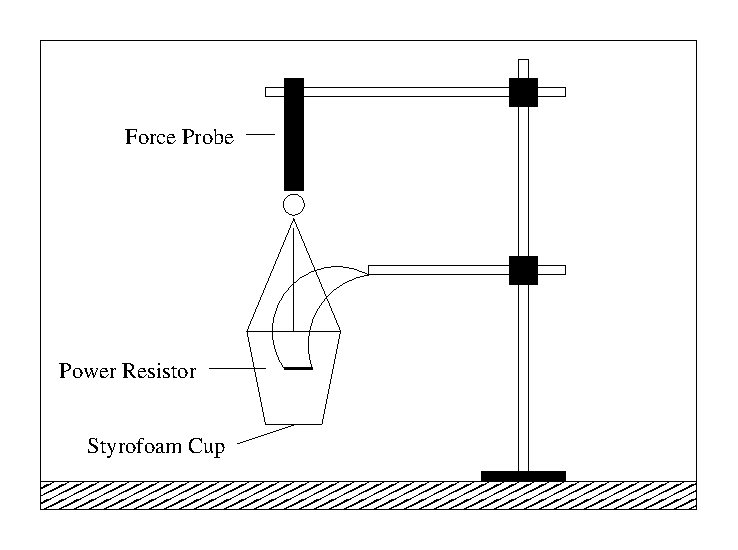
\includegraphics{heat_vap_nit_fig_1.eps}} \par}
\vspace{0.3cm}

\textbf{Introduction}

The experimental setup is shown in the figure above. The styrofoam
cup is filled with liquid nitrogen. The force transducer is used as
an electronic balance to measure the mass of the liquid nitrogen as
a function of time. The power resistor submerged in the liquid nitrogen
converts electrical energy into heat. The power, or rate at which
electrical energy is converted to heat, is determined from
the voltage and current.  The power supply will
display both of these values.
(Note: Power supply is
not shown in the figure.)

\textbf{Activity 1: Measuring the Heat of Vaporization of Nitrogen}

(a) Perform the following steps:

\begin{enumerate}
\item Remove the load from the force probe and press the TARE button.
\item Adjust the power resistor so that it is as far down in the cup as
possible without pushing down on the cup.
\item Fill the cup with liquid nitrogen.
\item Turn on the power supply.. Adjust the voltage and
current controls on the power supply so that the current is
2.0 A. Record the values of the current, I, and the voltage, V,
in the space below. Then turn off the power supply and refill the
cup with liquid nitrogen if necessary.\vspace{1in}

\item Open the \textit{NitrogenVap} application in the 132 Workshop folder
in the {\bf Start} menu.
\item The computer will measure the output of the force transducer every
second. Start collecting data by clicking on the Start button and
recording the force versus time for at least four minutes. When you
are finished make a linear fit to the data using the Fit menu. The
slope is related to the rate of evaporation of the liquid nitrogen.
Calculate the rate of mass loss from this measured slope and enter
the result in the space below. Print the graph of force versus time
and attach a copy to the unit. \vspace{0.75in}

\item Turn on the power supply and repeat step 6.
\item Turn off the power supply and repeat step 6.
\end{enumerate}
(b) Subtract the average of the absolute values of the two slopes
when power was off from the absolute value of the slope when power
was on. This is the net rate of evaporation caused by the energy supplied
to the heater.

(c) Calculate the heat of vaporization, L\( _{v} \), which is given
by

{\centering L\( _{v} \) = \( \frac{power\: to\: heater}{net\, rate\: of\: evaporation} \)=
\( \frac{VI}{net\, rate\: of\: evaporation} \)\par}
\vspace{30mm}

(d) Look up the accepted value for the heat of vaporization of nitrogen
and calculate the percent difference. Do the two values agree within
experimental uncertainties? Comment on possible sources of error.
\vspace{20mm}

(e) Was the temperature of the liquid nitrogen changing during this
experiment? Explain.
